\documentclass{article}
\usepackage[margin=1.5cm,bottom=2cm]{geometry}
\usepackage{fancyhdr}
\usepackage{graphicx}
\usepackage{amsmath}
\pagestyle{fancy}

\begin{document}
\fancyhead[L]{ 
\includegraphics[width=2cm]{au_logo.png} }
\fancyhead[R]{CPSC 2320: Computational Physics}
\fancyfoot[C]{\thepage}
\vspace*{0cm}
\begin{center}
	{\LARGE \textbf{Lab 1}}\\
	\vspace{0.25cm}
	%{\Large Due: Friday, September 18}
\end{center}

\section{The Quadratic Equation}
Write a program that solves an equation of the form 
\begin{equation*}
ax^2+bx+c=0
\end{equation*}
The general solution to this equation has two solutions:
\begin{equation*}
x=\frac{-b\pm\sqrt{b^2-4ac}}{2a}
\end{equation*}

Prompt the user to enter $a$,$b$,and $c$, and then solve for $x$. Print the solution to the console.

Your program must account for several possibilities:
\begin{enumerate}
	\item If $a=0$ the solution above is invalid. In this case, the equation is of the form 
	\begin{equation*}
	bx+c=0
	\end{equation*}
	which has the solution:
	\begin{equation*}
	x=-\frac{c}{b}
	\end{equation*}
	
	\item If both $a=0$ AND $b=0$, the equation cannot be solved. Either the user has entered a true statement ($c=0$) or not ($c!=0$). Test this and tell the user whether or not they have entered a true statement.
	
	\item Finally, the term under the square root ($b^2-4ac$), called the discriminant, might be negative. If this is the case, the solution is complex and cannot be solved. Print a message to the user stating that this is the case.
\end{enumerate}

\section{Projectile Motion}

\begin{figure}[ht!]
	\centering
	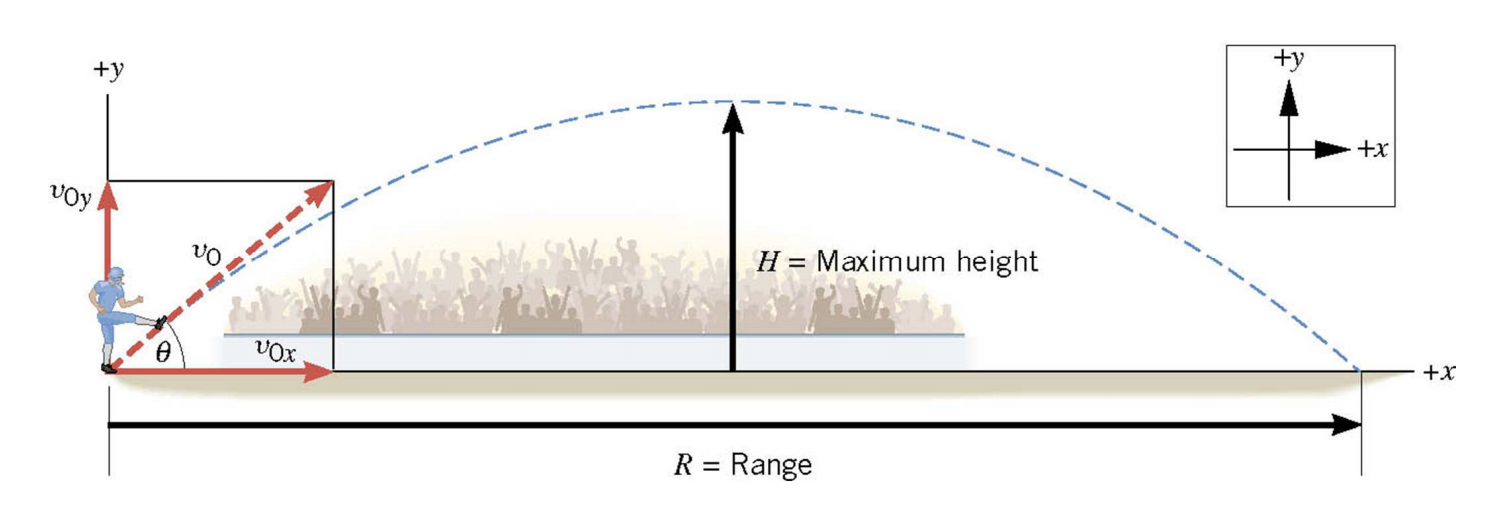
\includegraphics[width=0.75\textwidth]{football.png}
\end{figure}

A football place kicker kicks a football at an angle of $\theta$ degrees above the horizontal. The initial speed of the ball is $v_0=22$ m/s. Ignore air resistance and find the maximum height that the ball attains at the angles of 25, 45, 65, and 85 degrees.

The equation for maximum height is:
\begin{equation*}
H=\frac{v_0\sin^2{\theta}}{2g}
\end{equation*}
Where $g=-9.8$ m/$\mathrm{s}^2$.

Write a program which loops over the requested angles, calculates the max height $H$, and prints the output. Use the iomanip library from the discussed last week to format your output to a fixed width. See the sample output below:

\vspace{5cm}
\textbf{Sample Output}
\begin{table}[ht!]
	\begin{tabular}{cc}
		Angle [deg] & Max Height [m]\\
		25&4.41048\\
		45&12.3469\\
		65&20.2834\\
		85&24.5063\\
	\end{tabular}
\end{table}

\end{document}